%%
%% This is file `tikzposter-template.tex',
%% generated with the docstrip utility.
%%
%% The original source files were:
%%
%% tikzposter.dtx  (with options: `tikzposter-template.tex')
%%
%% This is a generated file.
%%
%% Copyright (C) 2014 by Pascal Richter, Elena Botoeva, Richard Barnard, and Dirk Surmann
%%
%% This file may be distributed and/or modified under the
%% conditions of the LaTeX Project Public License, either
%% version 2.0 of this license or (at your option) any later
%% version. The latest version of this license is in:
%%
%% http://www.latex-project.org/lppl.txt
%%
%% and version 2.0 or later is part of all distributions of
%% LaTeX version 2013/12/01 or later.
%%


\documentclass{tikzposter} %Options for format can be included here

\usepackage{todonotes}

\usepackage[tikz]{bclogo}
\usepackage{lipsum}
\usepackage{amsmath}

\usepackage{booktabs}
\usepackage{longtable}
\usepackage[absolute]{textpos}
\usepackage[it]{subfigure}
\usepackage{graphicx}
\usepackage{cmbright}
%\usepackage[default]{cantarell}
%\usepackage{avant}
%\usepackage[math]{iwona}
\usepackage[math]{kurier}
\usepackage[T1]{fontenc}


%% add your packages here
\usepackage{hyperref}
% for random text
\usepackage{lipsum}
\usepackage[english]{babel}
\usepackage[pangram]{blindtext}

\colorlet{backgroundcolor}{blue!10}

 % Title, Author, Institute
\title{What's Cooking}
\author{Siyu Chen}
\institute{ Xi'an Shiyou University, China \\
}
%\titlegraphic{logos/tulip-logo.eps}

%Choose Layout
\usetheme{Wave}

%\definebackgroundstyle{samplebackgroundstyle}{
%\draw[inner sep=0pt, line width=0pt, color=red, fill=backgroundcolor!30!black]
%(bottomleft) rectangle (topright);
%}
%
%\colorlet{backgroundcolor}{blue!10}

\begin{document}


\colorlet{blocktitlebgcolor}{blue!23}

 % Title block with title, author, logo, etc.
\maketitle

\begin{columns}
 % FIRST column
\column{0.5}% Width set relative to text width

%%%%%%%%%% -------------------------------------------------------------------- %%%%%%%%%%
 %\block{Main Objectives}{
%  	      	\begin{enumerate}
%  	      	\item Formalise research problem by extending \emph{outlying aspects mining}
%  	      	\item Proposed \emph{GOAM} algorithm is to solve research problem
%  	      	\item Utilise pruning strategies to reduce time complexity
%  	      	\end{enumerate}
%%  	      \end{minipage}
%}
%%%%%%%%%% -------------------------------------------------------------------- %%%%%%%%%%


%%%%%%%%%% -------------------------------------------------------------------- %%%%%%%%%%
\block{Introduction}{
    Asks you to predict the category of a dish's cuisine given a list of its ingredients. Test and submit the results to see the experimental score.
     
  \vspace{.5cm}
  \centering

  \begin{tabular}{ c | c | c }
    \toprule
    ID &  Cuisine    & Ingredients      \\
    \midrule
    10259 &  greek & romaine lettuce, black olives, grape tomatoes...\\
    25693 & southernus &plain flour, ground pepper, salt, tomatoes, g...\\
    20130  & filipino &eggs, pepper, salt, mayonaise, cooking oil, g... \\
    22213 & indian &water, vegetable oil, wheat, salt]\\
    13162& indian& black pepper, shallots, cornflour, cayenne pe...\\
    \bottomrule
\end{tabular}
  \vspace{.2cm}
  
}

%%%%%%%%%% -------------------------------------------------------------------- %%%%%%%%%%


%%%%%%%%%% -------------------------------------------------------------------- %%%%%%%%%%
\block{Data Analysis}{
    \begin{itemize}
        \item
        To better process the data, we need to do the following:
        
        \begin{itemize}
        \item
        Count the total data of training set and test set.
        
        train shape: 39774
        
        test shape: 9944
        \item
        Maximum Number of Ingredients in a Dish:  65
        \item
        Minimum Number of Ingredients in a Dish:  1
        
        train: 8529 
        
        test: 3310
       
        \end{itemize}
\end{itemize}


}
%%%%%%%%%% -------------------------------------------------------------------- %%%%%%%%%%


%%%%%%%%%% -------------------------------------------------------------------- %%%%%%%%%%

%\note{Note with default behavior}

%\note[targetoffsetx=12cm, targetoffsety=-1cm, angle=20, rotate=25]
%{Note \\ offset and rotated}

 % First column - second block


%%%%%%%%%% -------------------------------------------------------------------- %%%%%%%%%%
\block{Data Visualization}{
    
    \item Number of receipes by Cuisine. Italian cuisine dominates all cuisine.

\begin{tikzfigure}%[Overall architecture of \emph{GOAM} algorithm]
     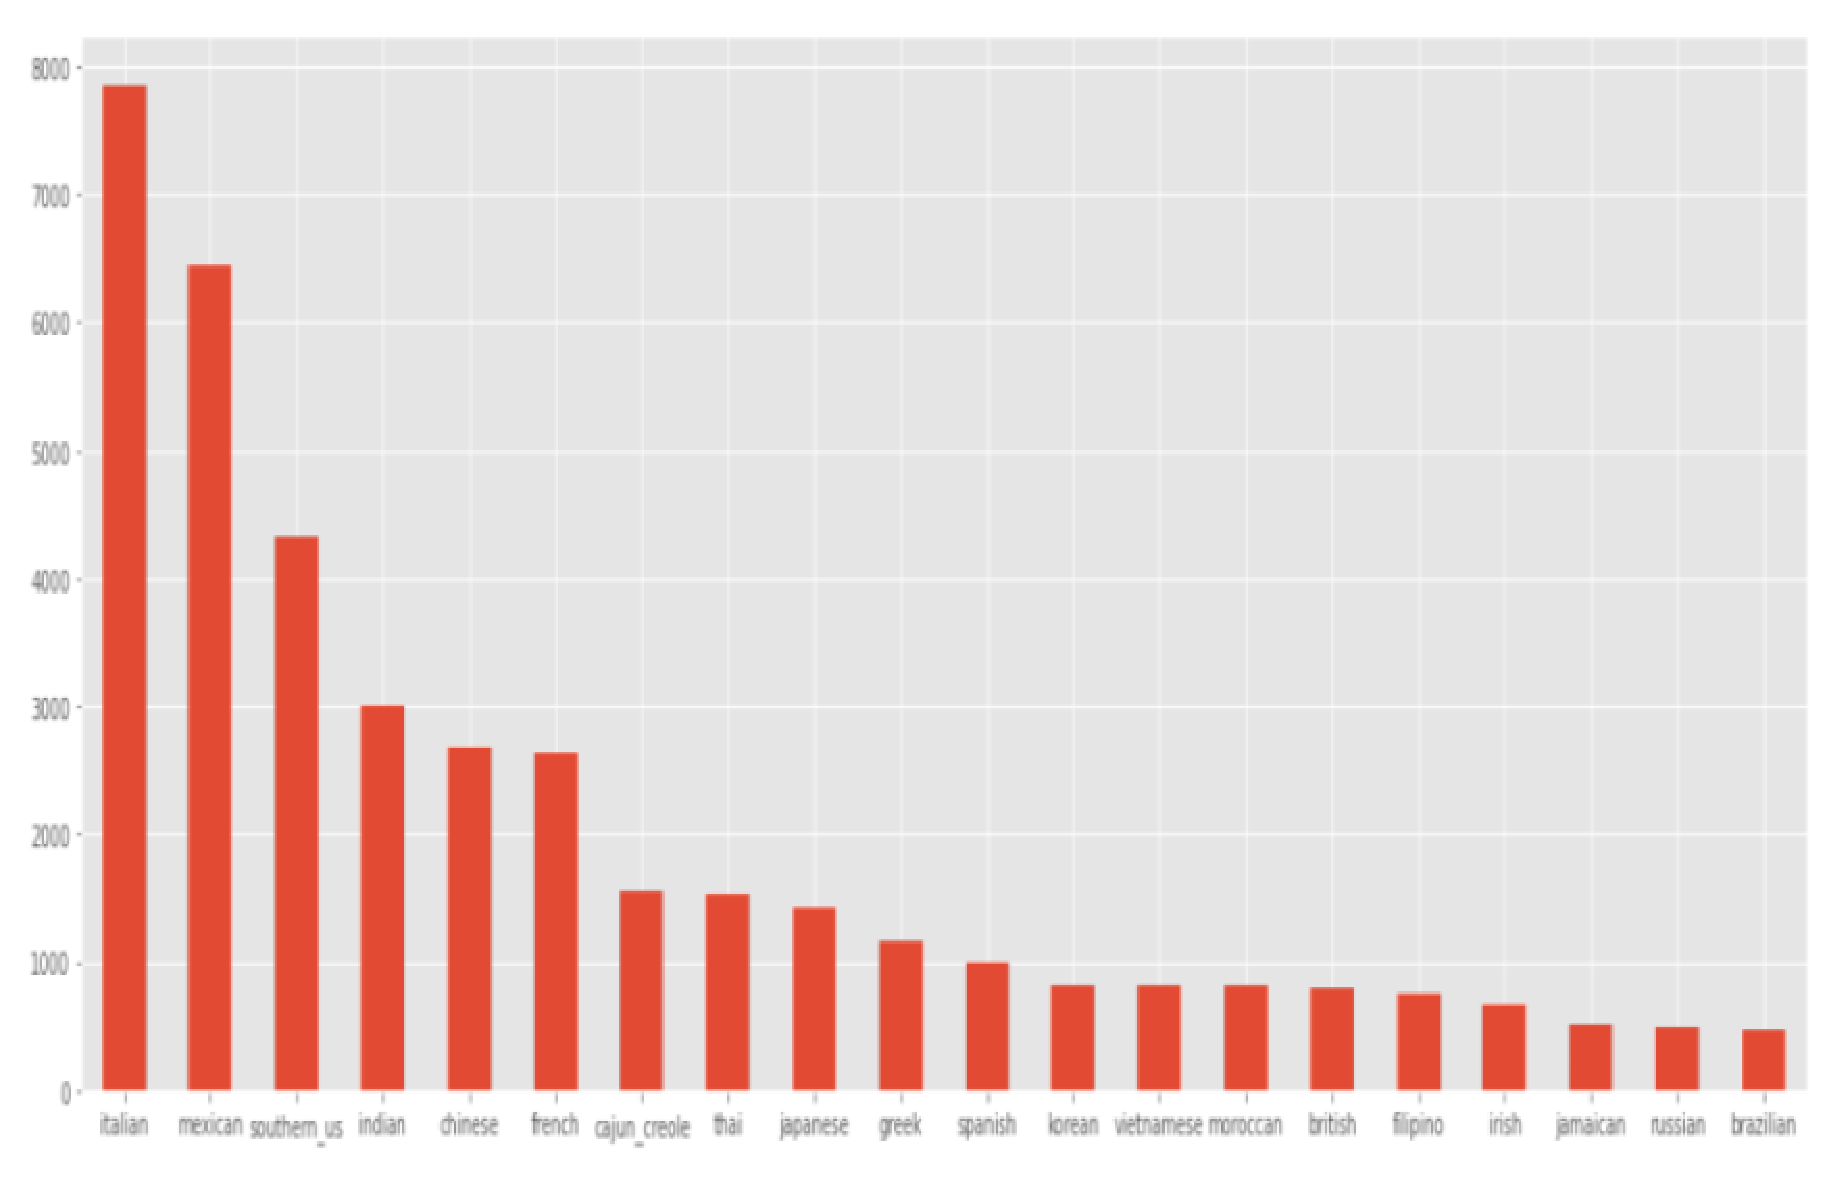
\includegraphics[width=0.6\linewidth]{figures/ns.eps}
        
    \end{tikzfigure}
    
        \item Ingredients in a dish distribution.
        \begin{tikzfigure}%[Overall architecture of \emph{GOAM} algorithm]
            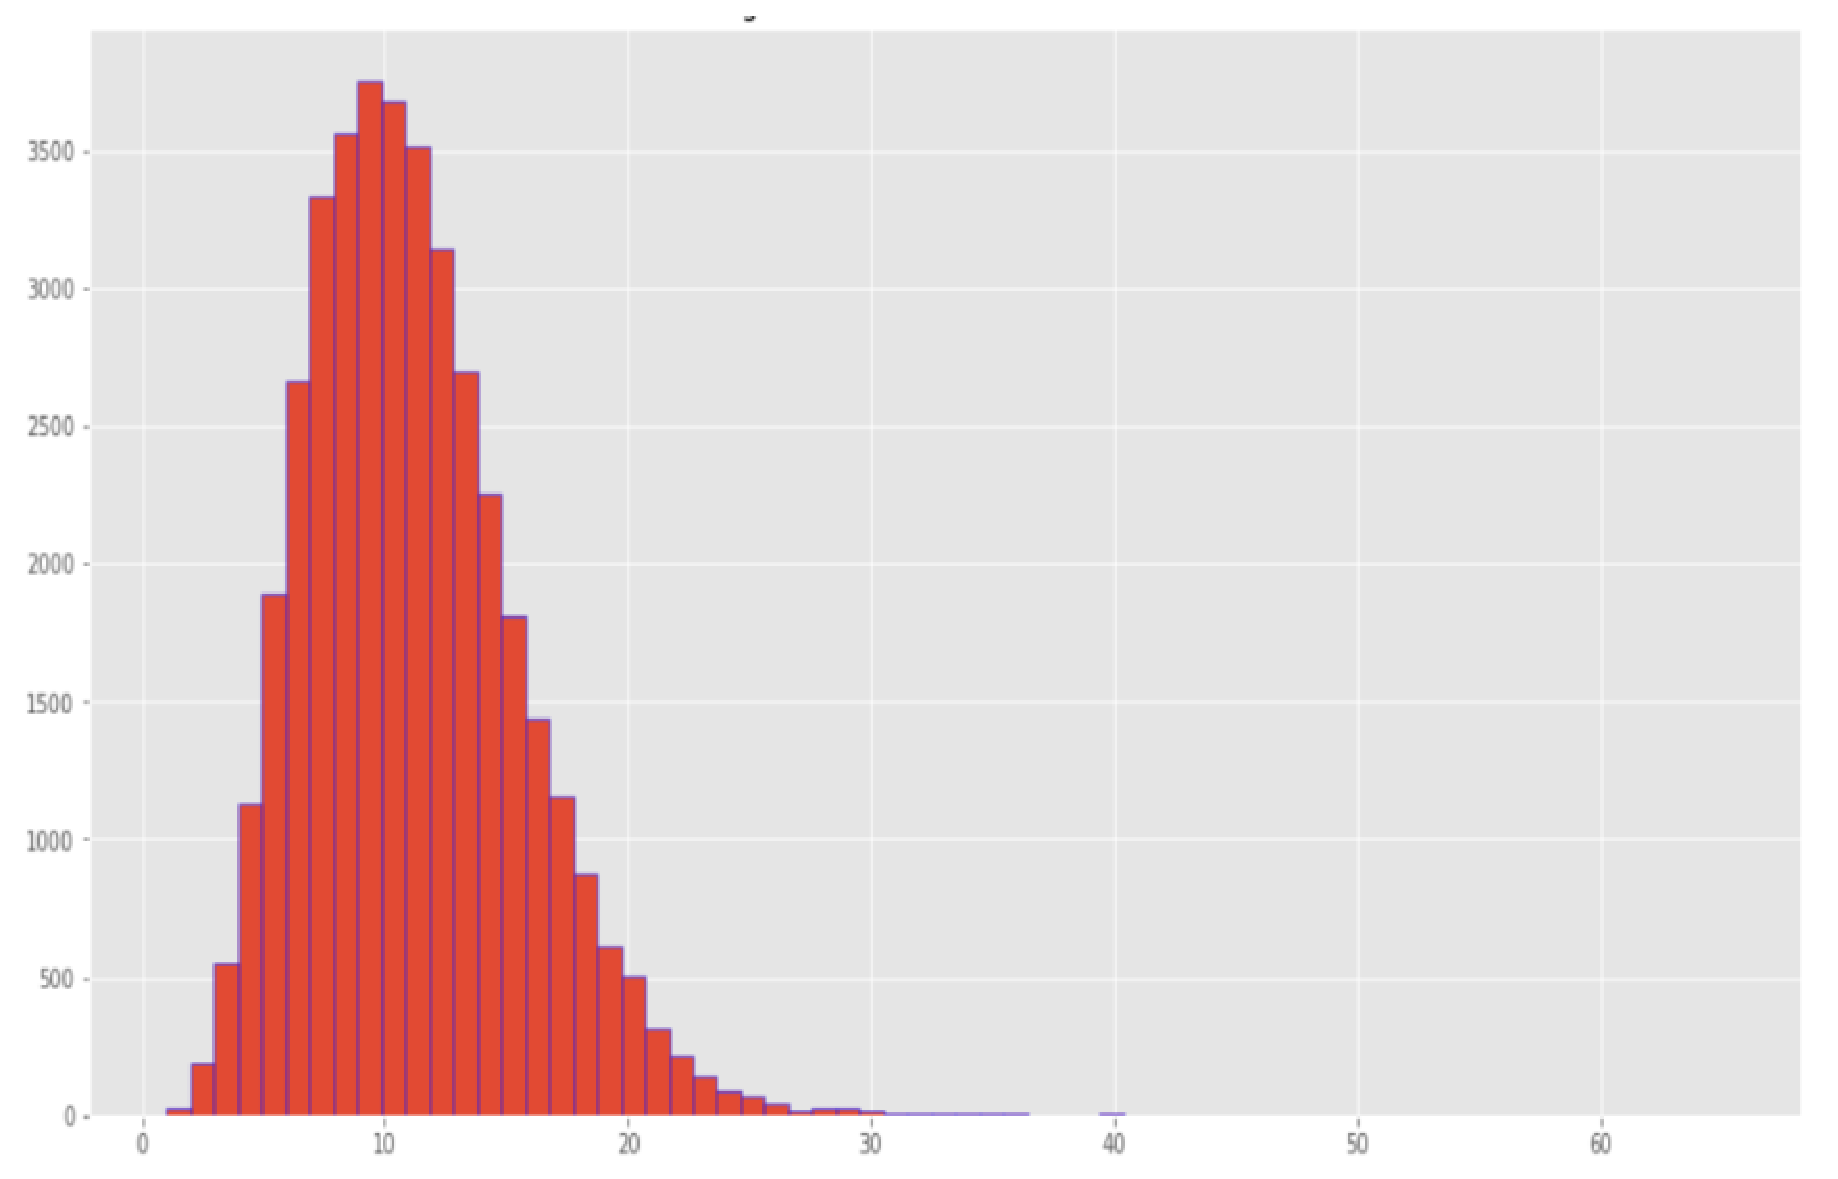
\includegraphics[width=0.6\linewidth]{figures/cu.eps}
        \end{tikzfigure}
        \item Salt is the largest share of all the Greek ingredients.
        \begin{tikzfigure}%[Overall architecture of \emph{GOAM} algorithm]
            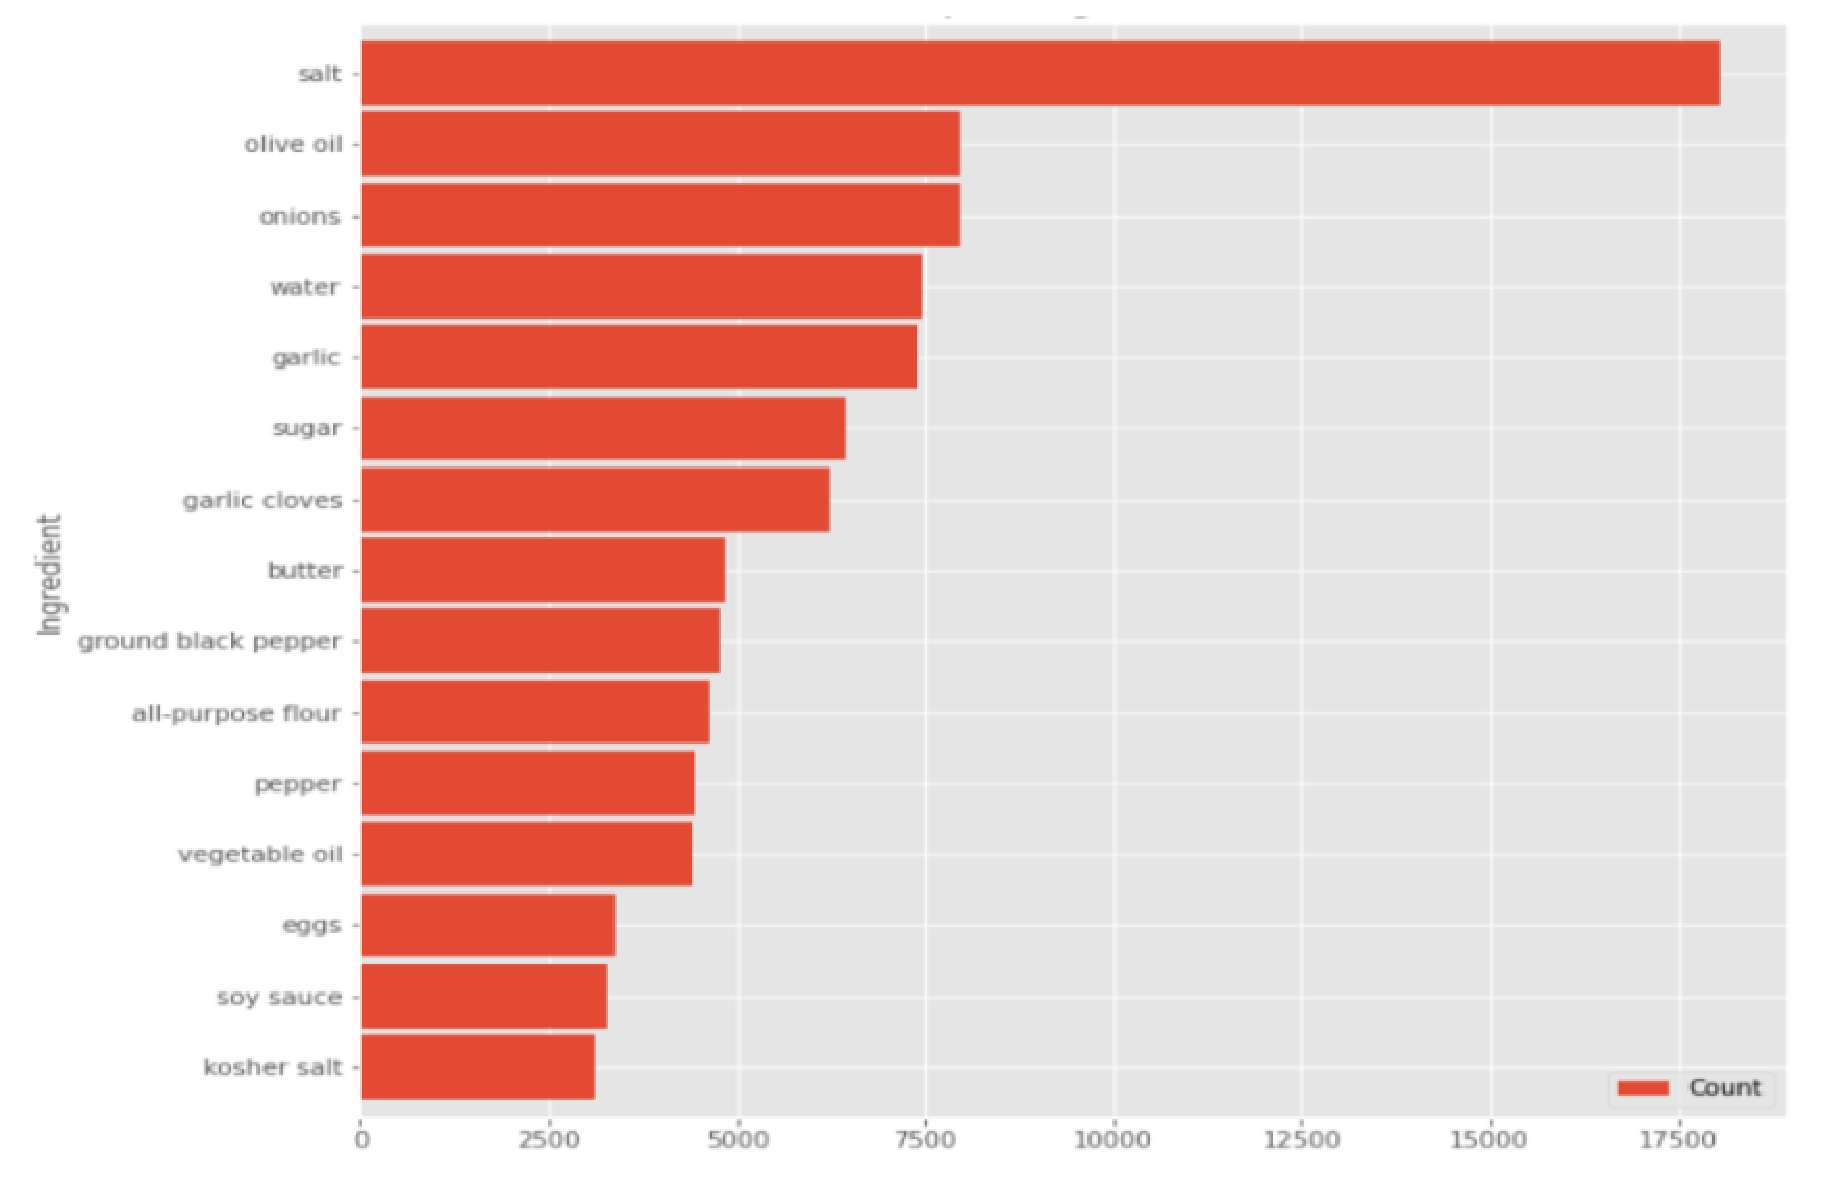
\includegraphics[width=0.6\linewidth]{figures/15.eps}
        \end{tikzfigure}
            %   1) Group Feature Extraction,
%    2) Outlying Degree Scoring, and
%    3) Outlying Aspects Identification.



}
%%%%%%%%%% -------------------------------------------------------------------- %%%%%%%%%%


% SECOND column
\column{0.5}
 %Second column with first block's top edge aligned with with previous column's top.

%%%%%%%%%% -------------------------------------------------------------------- %%%%%%%%%%
\block{NLP Analysis}{

    \begin{itemize}
        \item
        Model of TF-IDF algorithm
        
        \vspace{1.2cm}
        
        \begin{centering}
         
        $ TF-IDF (d, w) = TF (d, w) *IDF(w)$
        
        
        \end{centering}
        
        \begin{itemize}
        
        \item
        $TF(d,w)$ $\Leftrightarrow$ Frequency of occurrence of w in document d.
        \item
        $IDF(w) = log\frac{N}{N(w)}$
        \item
        N $\Leftrightarrow$ The total number of documents in a corpuss.
        \item
        N(w)$\Leftrightarrow$ How many documents does the w appear in.
        \end{itemize}
        \begin{itemize}
            \item
            Steps.
            
            \begin{itemize}
            \item
            The counting matrix of words is converted to TF-IDF representation, and then normalized.
            \item
            Scikit-learn provides a TfidfVectorizer class, which has the ability to remove common stop words (like a, the, and, or).
            \item
            TF-IDF tends to filter out common words and retain important words.
            
           
            \end{itemize}
        \end{itemize}
\end{itemize}

}
%%%%%%%%%% -------------------------------------------------------------------- %%%%%%%%%%
% Second column - first block


%%%%%%%%%% -------------------------------------------------------------------- %%%%%%%%%%
\block[titleleft]{Modeling}
{
    \begin{itemize}
    
        \smallskip
        \item
        Logistic Regressio\\
        Random seeds are not fixed and generate random sequences.\\
        Use the logistic regression model in sklearn.\\
        Score:0.787711182622687.
        \item
        \smallskip
        Ensemble Model\\
        Ensemble in Sklearn is called to integrate the two classifiers, logistic regression and SVM.\\
  in the way of soft voting, to show the accuracy.\\ 
  Score:0.8119469026548672. \\ 

  By comparing the accuracy of the two models, we found that the integrated accuracy is higher than that of a single classifier.
           
    \end{itemize}
}
%%%%%%%%%% -------------------------------------------------------------------- %%%%%%%%%%


% Second column - second block
%%%%%%%%%% -------------------------------------------------------------------- %%%%%%%%%%
\block[titlewidthscale=1, bodywidthscale=1]
{Create Submission}
{
    
    \begin{itemize}

        \item
        \smallskip
        \large
        {
        Output Dataframe:
        }
        
    \end{itemize}
  
    
    \vspace{.5cm}
\centering
\begin{tabular}{ c | c | c }
    \toprule
    &  ID    & Cuisine \\
    \midrule
    0 &  18009    &  british  \\
    
    1 &  28583    &  southern\_us \\
    
    2 &   41580    &  italian \\
    3 &   29752    &  cajun\_creole \\
    4 &   35687    &  italian    \\
    5 &   38527    &  southern\_us\\
    \bottomrule
\end{tabular}



}
%%%%%%%%%% -------------------------------------------------------------------- %%%%%%%%%%
\block{Reflection and Summary}{
    \begin{itemize}
        \item
        Disadvantages and optimizations:
        
        \begin{itemize}
        \item
        Dishes can contain a variety of ingredients, and the same ingredients may vary in number and number, so the integredients need to be filtered.
        \item
        KNN mainly depends on the surrounding limited adjacent samples, rather than on the method of discriminating class domain to determine the category.
        \item
        KNN basically does not learn, resulting in a slower prediction speed than logistic regression and other algorithms.
        
       
        \end{itemize}
\end{itemize}


}

% Bottomblock
%%%%%%%%%% -------------------------------------------------------------------- %%%%%%%%%%


%\note[targetoffsetx=8cm, targetoffsety=-10cm,rotate=0,angle=180,radius=8cm,width=.46\textwidth,innersep=.1cm]{
%Acknowledgement
%}

%\block[titlewidthscale=0.9, bodywidthscale=0.9]
%{Acknowledgement}{
%}
%%%%%%%%%% -------------------------------------------------------------------- %%%%%%%%%%

\end{columns}


%%%%%%%%%% -------------------------------------------------------------------- %%%%%%%%%%
%[titleleft, titleoffsetx=2em, titleoffsety=1em, bodyoffsetx=2em,%
%roundedcorners=10, linewidth=0mm, titlewidthscale=0.7,%
%bodywidthscale=0.9, titlecenter]

%\colorlet{noteframecolor}{blue!20}
\colorlet{notebgcolor}{blue!20}
\colorlet{notefrcolor}{blue!20}
\note[targetoffsetx=-13cm, targetoffsety=-12cm,rotate=0,angle=180,radius=8cm,width=.96\textwidth,innersep=.4cm]
{
\begin{minipage}{0.3\linewidth}
\centering

\includegraphics[width=24cm]{logos/tulip-wordmark.eps}
\end{minipage}
\begin{minipage}{0.7\linewidth}
{ \centering
What's Cooking,
  14/1/2021, xi'an, China
}
\end{minipage}
}
%%%%%%%%%% -------------------------------------------------------------------- %%%%%%%%%%


\end{document}

%\endinput
%%
%% End of file `tikzposter-template.tex'.
